\section{Проекційні методи. Метод моментів. \texorpdfstring{\\}{} Метод Бубнова-Гальоркіна}
\subsection{Постановка задачі і допоміжні твердження}
Розгялнемо рівняння
\begin{equation}
    \label{eq:1.1}
    A u = f,
\end{equation}
де $A: E \to F$ --- лінійний, діє на парі лінійниї нормованих просторів, $D(A) \subseteq E$, $R(A) \subseteq F$. \medskip

Розглянемо послідовність підпросторів $E_n \subseteq D(A)$, $F_n \subseteq F$. Введемо лінійні \textit{оператори проектування} $P_n: F \to F_n$ такі, що $P_n^2 = P_n$. Тоді можна розглянути послідовність рівнянь
\begin{equation}
    \label{eq:1.2}
    P_n (A u_n - f) = 0,
\end{equation}
із розв'язками $u_n \in E_n$. Враховуючи лінійність операторів проектування маємо $P_n (A u_n) = P_n f$. Зрозуміло, що у залежності від вибору $E_n, F_n, P_n$ отримаємо різні \textit{проекційні розв'язки} $u_n$. \medskip

Нехай надалі $E, F$ --- гільбертові простори.

\begin{definition}
    Розглянемо лінійно незалежні системи функцій $\{\phi_i\} \in D(A)$ і $\{\psi_i\} \in F$. Система $\{\phi_i\}$ називається \textit{координатною}, а система $\{\psi_i\}$ --- \textit{проекційною}.
\end{definition}

У якості $E_n$ візьмемо $\mathcal{L}(\phi_1, \ldots, \phi_n)$, а в якості $F_n$ --- $\mathcal{L}(\psi_1, \ldots, \psi_n)$.

\begin{proposition}
    Тоді для виконання умови $P_n^2 = P_n$ достатньо, аби $P_n|_{F_n}$ був тотожнім оператором.
\end{proposition}
\begin{proof}
    Справді, тоді $P_n f = f_n \in F_n$ і $P_n^2 f = P_n f_n = f_n$.
\end{proof}
\subsection{Метод моментів}
Розв'язок задачі \eqref{eq:1.2} будемо шукати у вигляді
\begin{equation}
    \label{eq:1.3}
    u_n = \sum_{i = 1}^n c_i \phi_i.
\end{equation}

\begin{lemma}
    Для довільного елементу $\psi \in F$ рівність
    \begin{equation}
        \label{eq:1.4}
        P_n \psi = 0
    \end{equation}
    та система рівностей
    \begin{equation}
        \label{eq:1.5}
        (\psi, \psi_j) = 0, \quad j = \overline{1, n}
    \end{equation}
    рівносильні.
\end{lemma}
\begin{proof}
    Нехай виконується \eqref{eq:1.4}, тоді маємо 
    \begin{equation*}
        (\psi, \psi_j) = (\psi, P_n \psi_j) = (P_n \psi, \psi_j) \overset{\eqref{eq:1.4}}{=} (0, \psi_j) = 0,
    \end{equation*}
    тому виконується \eqref{eq:1.5}. \medskip
    
    В інший бік: нехай виконується \eqref{eq:1.5}, тоді 
    \begin{equation*}
        \begin{aligned}
            (P_n \psi, P_n \psi) &= \left(P_n \psi, \sum_{j = 1}^n a_j \psi_j \right) = \left(\psi, \sum_{j = 1}^n a_j P_n \psi_j \right) = \\
            &= \left(\psi, \sum_{j = 1}^n a_j \psi_j \right) = \sum_{j = 1}^n \overline{a_j} (\psi, \psi_j) \overset{\eqref{eq:1.5}}{=} 0.
        \end{aligned}
    \end{equation*}
\end{proof}
\begin{remark}
    Тут ми скористалися самоспряженістю оператора проектування, хоча і не довели її.
\end{remark}
\begin{exercise}
    Доведіть, що $P_n$ --- самоспряжений оператор.
\end{exercise}
\begin{solution}
    Нехай $x = \psi_x + f_x$, $y = \psi_y + f_y$ де $\psi_x, \psi_y \in F_n$ а $f_x, f_y \in F_n^\perp$, тоді 
    \begin{equation*}
        (P_n x, y) = (\psi_x, \psi_y + f_y) = (\psi_x, \psi_y) = (\psi_x + f_x, \psi_y) = (x, P_n y).
    \end{equation*}
\end{solution}
\begin{remark}
    Тут ми скористалися тим, що $F = F_n \oplus F_n^\perp$. Це, взагалі кажучи, не так, якщо $F_n$ нескінченновимірний, але ми не оперуємо з такими просторами, тому все законно.
\end{remark}

Таким чином, ми можемо знайти розв'язок 
\begin{equation}
    \label{eq:1.6}
    (A u_n - f, \psi_j) = 0, \quad j = \overline{1,n}.
\end{equation}
Розв'язок шукаємо у вигляді \eqref{eq:1.3} і підставляємо в \eqref{eq:1.6}:
\begin{equation}
    \label{eq:1.7}
    \sum_{i = 1}^n c_i (A \phi_i, \psi_i) = (f, \psi_j), \quad j = \overline{1, n}.
\end{equation}
Це і є \textbf{метод моментів}.

\begin{algorithm} $\left.\right.$
    \label{algorithm:1.7}
    \begin{enumerate}
        \item Обираємо повну систему лінійно-незалежних функцій $\{\phi_i\} \in D(A)$;
        \item Обираємо замкнену систему лінійно-незалежних функцій $\{\psi_i\} \in F$;
        \item Шукаємо розв'язки у вигляді $u_n = \sum_{i = 1}^n c_i \phi_i$, отримуємо СЛАР \eqref{eq:1.7}.
    \end{enumerate}
\end{algorithm}
\subsection{Метод Бубнова-Гальоркіна}
\begin{remark}
    Якщо $\psi_j = \phi_j$, то отримуємо метод Бубнова-Гальоркіна. Для нього система має вигляд 
    \begin{equation*}
        (A u_n - f, \psi_j) = 0,
    \end{equation*}
    або, у розгорнутому вигляді,
    \begin{equation}
        \label{eq:1.8}
        \sum_{i = 1}^n c_i (A \phi_i, \phi_j) = (f, \phi_j), \quad j = \overline{1, n}.
    \end{equation}
\end{remark}

\begin{remark}
    У книжці Ляшка, Макарова, і Скоробагатько ``Методы вычис\ldots'' наведена загальна теорема про збіжність.
\end{remark}

\section{Виділення самоспряженого оператору. \texorpdfstring{\\}{} Узагальнений розв'язок}
\subsection{Основні визначення}
Для ситуації, коли
\begin{equation}
    \label{eq:2.1}
    A = A_0 + B,
\end{equation}
де $A_0$ --- самоспряжений додатновизначений оператор введемо розглянемо рівняння
\begin{equation}
    \label{eq:2.2}
    [u, v] + (B u, v) = (f, v), \quad \forall v \in H_{A_0},
\end{equation}
де
\begin{definition}
    $H_{A_0}$ --- \textit{енергетичний простір} зі скалярним добутком 
    \begin{equation*}
        [u, v] = (A_0 u, v) 
    \end{equation*}
    і породженю ним нормою
    \begin{equation*}
        \|u\|_{A_0} = |[u]| = \sqrt{[u, u]}.
    \end{equation*}
\end{definition}
\begin{remark}
    Енергетичний простір у чомусь ідеологічно схожий на слабкий топологічний простір.
\end{remark}
\subsection{Збіжність методу Бубнова-Гальоркіна}
Тоді алгоритм Бубнова-Гальоркіна набуває вигляду
\begin{algorithm}[Бубнова-Гальоркіна]
    $\left.\right.$
    \begin{enumerate}
        \item Обираємо повну систему лінійно-незалежних функцій $\{\phi_i\} \in H_{A_0}$;
        \item $H_n = \mathcal{L}(\phi_1, \ldots, \phi_n)$;
        \item Шукаємо розв'язки у вигляді $u_n = \sum_{i = 1}^n c_i \phi_i$.
    \end{enumerate}
\end{algorithm}

У такій ситуації маємо
\begin{equation}
    \label{eq:2.3}
    [u_n, \phi_j] + (B u_n, \phi_j) = (f \phi_j),
\end{equation}
тобто
\begin{equation}
    \label{eq:2.4}
    L \vec{c} = \vec{f},
\end{equation}
де
\begin{equation*}
    L_{ij} = [\phi_i, \phi_j] + (B \phi_i, \phi_j),  \quad \vec{f} = (f, \phi_j), \quad i, j = \overline{1,n}.
\end{equation*}

\begin{definition}
    Послідовність просторів $E_n$ називається \textit{гранично щільною} в $E$, якщо 
    \begin{equation}
        \label{eq:2.5}
        \lim_{n \to \infty} \rho(\phi, u_n) = \lim_{n \to \infty} \inf_{u_n \in E_n} \|\phi - u_n\| = 0, \quad \forall f \in E.
    \end{equation}
\end{definition}
\begin{definition}
    Оператор $A$ називається \textit{майже всюди неперервним}, якщо $A = A_1 + A_2$, де $\|A_2\| \le \epsilon$, а \[A_1 u = \sum_{i = 1}^n (u, \phi_i) \psi_i.\]
\end{definition}

\begin{theorem}
    Нехай \eqref{eq:1.1} має єдиний розв'язок, $A_0^{-1} B$ є майже всюди неперервним, а $H_n$ --- гранично щільною в $H_{A_0}$, тоді алгоритм Бубнова-Гальоркіна генерує єдиний розв'язок задачі \eqref{eq:2.4}, причому послідовність цих розв'язків збігається до розв'язку задачі \eqref{eq:1.1} у просторі $H_{A_0}$.
\end{theorem}
\subsection{Приклади}
\begin{example}
    Розглянемо найпростіше диференціальне рівняння
    \begin{equation}
        \label{eq:2.6}
        -(ku')'-pu'+qu=f,\quad a<x<b
    \end{equation}
    з крайовими умовами першого роду
    \begin{equation}
        \label{eq:2.7}
        u(a)=u(b)=0.
    \end{equation}
\end{example}
Його класичний двічі неперервно диференційовний (з $C^2([a,b])$) розв'язок існує за умов $k(x) \ge k_0 > 0$, $k \in C^1((a,b))$, $p,q,f \in C(a,b)$. \medskip

Розгялнемо тепер системи функцій $\phi_i,\psi_i$:
\begin{enumerate}
    \item $\phi_i = (x - a)^i (b - x)$;
    \item $\phi_i = \sin \left( \dfrac{x - a}{b - a} i \pi \right)$;
\end{enumerate}
і $\psi_i = x^{i - 1}$, $i = \overline{1,n}$. \medskip

Тоді у класичному методі моментів будемо мати
\begin{equation*}
    (u,v)=\int_a^b u(x)v(x) \diff x,
\end{equation*}
і
\begin{equation}
    \label{eq:2.8}
    \sum_{i=1}^n c_i \int_a^b (-(k\phi_i')'-p \phi_i' + q\phi_i)\psi_j \diff x = \int_a^b f \psi_j \diff x, \quad j = \overline{1,n}.
\end{equation}

\begin{remark}
    У методі Бубнова-Гальоркіна матимемо
    \begin{equation*}
        \sum_{i=1}^n c_i \int_a^b (-(k\phi_i')'-p \phi_i' + q\phi_i)\phi_j \diff x = \int_a^b f \phi_j \diff x, \quad j = \overline{1,n}.
    \end{equation*}
\end{remark}

\begin{example}
    Нехай $f \in L_2$ ($p, q, k' \in L_2)$, тоді отримуємо  $W_2^2((a,b))$.
\end{example}

\begin{example}
    Нехай $f \in W_2^{-1}$, тоді  $u \in W_2^1((a,b))$, а $D(A) = \{u \in W_2^1([a,b]), u(a) = u(b) = 0\}$.
\end{example}
\begin{remark}
    Оскільки тепер функція має лише першу похідну, то необхідно переписати \eqref{eq:2.8}:
    \begin{equation*}
        \sum_{i=1}^n c_i \int_a^b (k \phi_i'\phi_j' - p \phi_i' \phi_j + q \phi_i \phi_j) \diff x - \left. k \phi_i' \phi_j \right|_{x = a} + \left. k \phi_i' \phi_j \right|_{x = b} = \int_a^b f \phi_j \diff x.
    \end{equation*}
\end{remark}
\begin{remark}
    Якщо $f \in W_2^{-1}$, то $f = f_0 - \frac{\diff f_1}{\diff x}$, де $f_0, f_1 \in L_2$, тому базисними функціями для цієї ситуації можна взяти ``штафетини'':
    \begin{figure}[H]
        \centering
        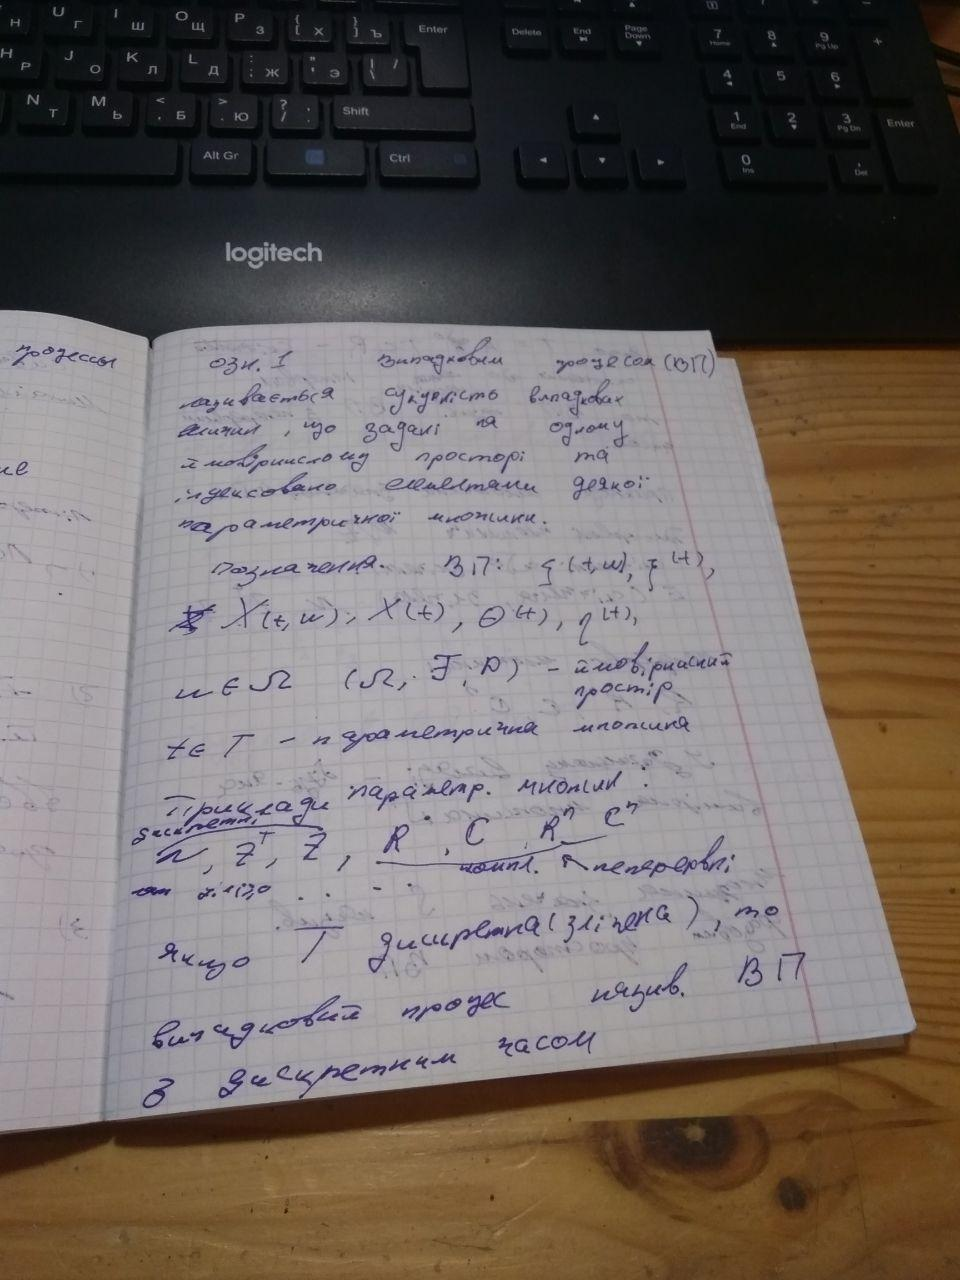
\includegraphics[width=.5\textwidth]{{img/01/01}.mps}
        \caption{``штафетина'' від $x_{i-1}$ до $x_i$.}
    \end{figure}
\end{remark}